\section{Auswertung}
\label{sec:Auswertung}


Die Graphen werden sowohl mit Matplotlib \cite{matplotlib} als auch NumPy \cite{numpy} erstellt. Die Fehlerrechnung wird mithilfe von Uncertainties \cite{uncertainties} durchgeführt.
\subsection{Bestimmung des brechenden Winkels $\phi$}

Die für die Berechnung des brechenden Winkels $\phi$ zwischen den Seiten des Prismas benötigten Werte sind in Tabelle \ref{tab:1} zu finden.
$\phi$ berechnet sich dabei nach Gleichung \eqref{eq:phi}.
Damit ergibt sich
\[
\bar{\phi} = \SI{59,99(2)}{\degree}\text{.}
\]
Der Wert bestimmt sich dabei über die Formel des Mittelwerts
\[
\bar{\phi} = \frac{1}{N}\sum_.{n=1}^N \phi_.n
\]
und der Fehler über die Formel zur Berechnung der Standardabweichung
\[
\sigma_.{\phi}=\sqrt{\frac{1}{N^2-N}\sum_.{n=1}^N \left(\phi_.n-\bar{\phi}\right)^2}\text{.}
\]
\begin{table}
	\centering
	\caption{Messwerte zur Bestimmung des Winkels $\phi$}
	\label{tab:tabphi}
	\sisetup{table-format=1.2}
	\begin{tabular}{S[table-format=3.1]S[table-format=3.1]S[table-format=2.2]}
		\toprule
		{$\phi_.r/\si{\degree}$} & {$\phi_.l/\si{\degree}$} & {$\phi/\si{\degree}$} \\
		\midrule
		217.5 & 97.5 & 60.00 \\
		218.9 & 98.9 & 60.00 \\
		219.4 & 99.6 & 59.90 \\
		220.4 & 100.5 & 59.95 \\
		221.9 & 101.7 & 60.10 \\
		222.3 & 102.2 & 60.05 \\
		223.5 & 103.7 & 59.90 \\
		\bottomrule
	\end{tabular}

	\label{tab:1}
\end{table}

\subsection{Bestimmung des Brechungswinkels $\eta$ und des Brechungsindex $n$}
Die zur Berechnung von $\eta$ und $\phi$ erhobenen Daten befinden sich in Tabelle \ref{tab:2}.
Dabei errechnet sich $\eta$ nach Gleichung \eqref{eq:eta} und $n$ nach Gleichung \eqref{eq:n}.
Der Fehler von $n$ berechnet sich dabei nach der Gauß'schen Fehlerfortpflanzung zu
\[
\sigma_.n=\frac{\partial n}{\partial \phi}\cdot \sigma_.{\phi}\text{.}
\]
\begin{table}
	\centering
	\caption{Messwerte zur Bestimmung des Winkels $\eta$ und des Brechungsindex $n$}
	\label{tab:tabn}
	\sisetup{table-format=1.2}
	\begin{tabular}{S[table-format=3.1]S[table-format=3.1]S[table-format=3.1]S[table-format=2.1]S[table-format=1.2]@{${}\pm{}$}S[table-format=1.5]}
		\toprule
		{$\lambda/10^{-9}\si{\metre}$} & {$\Omega_.r/\si{\degree}$} & {$\Omega_.l/\si{\degree}$} & {$\eta/\si{\degree}$} &  \multicolumn{2}{c}{$n$} \\
		\midrule
		404.7 & 215.3 & 105.0 & 69.7 & 1.81 & 0.00056 \\
		407.8 & 215.4 & 104.9 & 69.5 & 1.81 & 0.00056 \\
		435.8 & 216.3 & 104.0 & 67.7 & 1.80 & 0.00055 \\
		480.0 & 217.2 & 103.2 & 66.0 & 1.78 & 0.00054 \\
		491.6 & 217.3 & 102.9 & 65.6 & 1.78 & 0.00053 \\
		508.6 & 217.8 & 102.4 & 64.6 & 1.77 & 0.00053 \\
		546.1 & 218.2 & 102.0 & 63.8 & 1.76 & 0.00052 \\
		577.0 & 218.5 & 101.7 & 63.2 & 1.76 & 0.00052 \\
		579.1 & 218.6 & 101.6 & 63.0 & 1.76 & 0.00052 \\
		643.8 & 219.2 & 101.1 & 61.9 & 1.75 & 0.00051 \\
		\bottomrule
	\end{tabular}

	\label{tab:2}
\end{table}

\subsection{Dispersionsgleichung}
\label{sec:Dispersion}
Um zu überprüfen welche Dispersionsgleichung besser zu den Messdaten passt, wird Gleichung \eqref{eq:n^2 für l>>l1} bis zur 2. und zur 4. Potenz entwickelt so wie Gleichung \eqref{eq:n^2 für l<<l1} bis zur 2. 
Mittels der Regressionen
\begin{equation}
n^2_.2 (\lambda)=A_.{0_.2}+\frac{A_.{2_.2}}{\lambda^2},\label{eq:reg2}
\end{equation}
\begin{equation}
n^2_.4 (\lambda)=A_.{0_.4}+\frac{A_.{2_.4}}{\lambda^2}+\frac{A_.{4_.4}}{\lambda^4}\label{eq:reg4}
\end{equation}
und
\begin{equation}
n'^2(\lambda)=A_.0'-A_.2'\cdot \lambda^2\label{eq:reg'}
\end{equation}
werden die Koeffizienten bestimmt zu
\begin{align*}
A_.{0_.2}&= 2,914\pm 0,004\text{,} \\
A_.{2_.2}&= (5,96\pm 0,1)\cdot 10^{-14}\text{,} \\
A_.{0_.4}&= 2,92\pm 0,02 \text{,}\\
A_.{2_.4}&= (5,8\pm 0,9)\cdot 10^{-14}\text{,} \\
A_.{4_.4}&= (0,2\pm 1,0)\cdot 10^{-27}\text{,} \\
A_.0'  &= 3,40\pm 0,03\text{,} \\
A_.2'  &= (9,0\pm 0,9)\cdot 10^{11}\text{.} \\
\end{align*}
Die Abweichungsquadrate $s^2$ werden bestimmt über 
\begin{equation}
s^2_.n = \frac{1}{z-2}\sum_.{i=1}^z \left(n^2(\lambda_.i)-A_.0-\frac{A_.2}{\lambda^2_.i}\right)^2
\end{equation}
und
\begin{equation}
s^2_.n = \frac{1}{z-2}\sum_.{i=1}^z \left(n^2(\lambda_.i)-A_.0' +A_.2\cdot\lambda^2_.i\right)^2,
\end{equation}
wobei $z$ die Anzahl der Messdaten ist und $\lambda_.i$ und $n(\lambda_.i)$ die Wellenlängen mit den dazugehörigen Brechungsindizes aus Tabelle \ref{tab:2} sind.
Damit ergibt sich:
\begin{align*}
s^2_.{n_.2}&=1,541\cdot 10^-5\text{,} \\
s^2_.{n_.4}&=1,536\cdot 10^-5\text{,} \\
s^2_.{n'}&=5,041\cdot 10^-4\text{.} \\
\end{align*}
Die Graphen zu den verschiedenen Ausgleichskurven sind in den Abbildungen \ref{fig:reg2} bis \ref{fig:reg'} zu sehen.
Da die Regression \eqref{eq:reg4} die kleinsten Abweichungsquadrate liefert, wird im folgenden diese zur Berechnung verwendet.

\begin{figure}
\centering
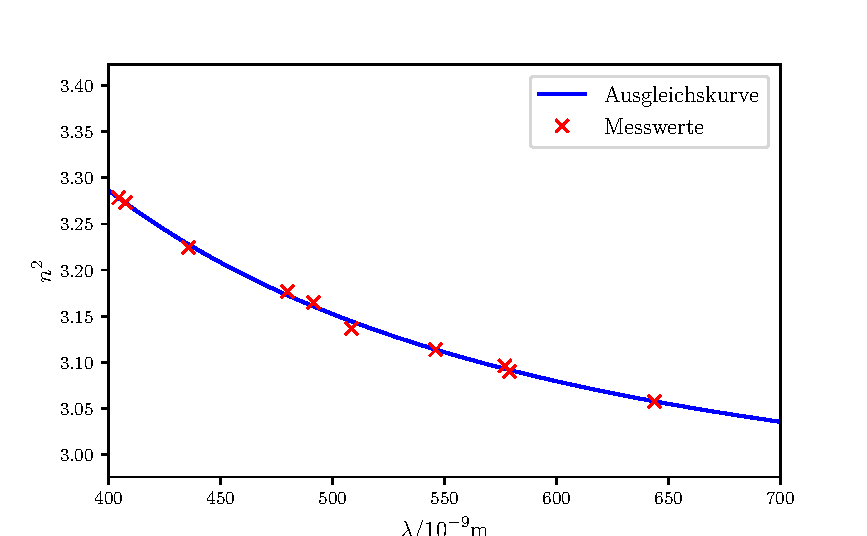
\includegraphics[width=\linewidth-70pt,height=\textheight-70pt,keepaspectratio]{content/images/Graph11.pdf}
\caption{Messwerte mit der Regression \eqref{eq:reg2}}
\label{fig:reg2}
\end{figure}

\begin{figure}
\centering
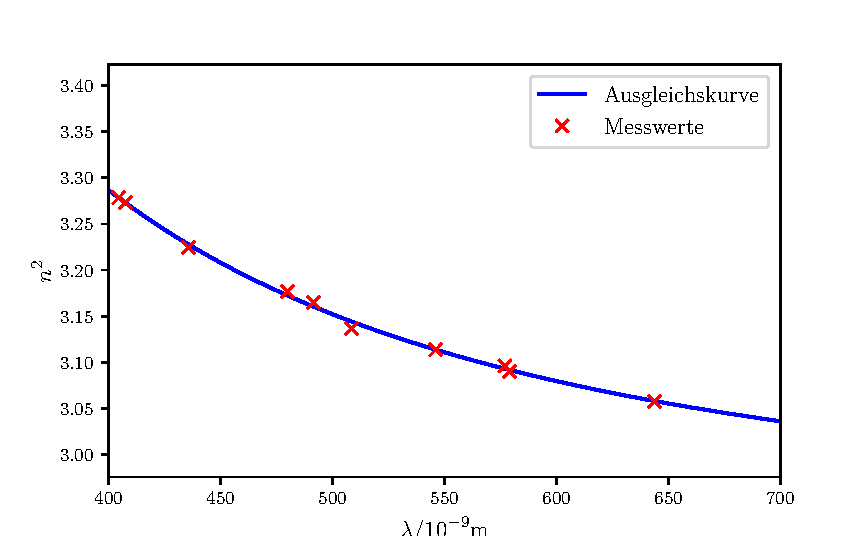
\includegraphics[width=\linewidth-70pt,height=\textheight-70pt,keepaspectratio]{content/images/Graph11.4.pdf}
\caption{Messwerte mit der Regression \eqref{eq:reg4}}
\end{figure}

\begin{figure}
\centering
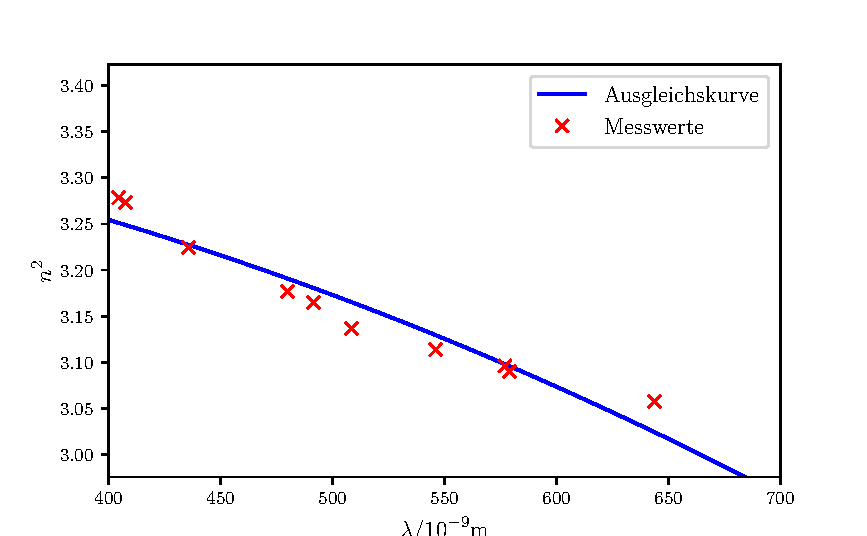
\includegraphics[width=\linewidth-70pt,height=\textheight-70pt,keepaspectratio]{content/images/Graph11a.pdf}
\caption{Messwerte mit der Regression \eqref{eq:reg'}}
\label{fig:reg'}
\end{figure}

\subsection{Bestimmung der Absorptionsstelle}

Durch einen Vergleich der Koeffizienten in Gleichung \eqref{eq:n^2 für l>>l1} lässt sich für die Absorptionsstelle $\lambda_.1$ herleiten:
\[
\lambda_.1 = \sqrt{\frac{A_.2}{A_.0-1}}=\SI{176,5(15)e-9}{\metre}\text{.}
\]
Der Fehler berechnet sich dabei über
\[
\sigma_.{\lambda} =\sqrt{\left(\frac{\partial \lambda_.1}{\partial A_.0}\right)^2\cdot\sigma^2_.{A_.0}+\left(\frac{\partial\lambda_.1}{\partial A_.2}\right)^2\cdot\sigma^2_.{A_.2}},
\]
wobei die Fehler $\sigma_.{A_.0}$ und $\sigma_.{A_.2}$ aus Abschnitt \ref{sec:Dispersion} bekannt sind.

\subsection{Abbe-Zahl}
Für die Fraunhofer-Wellenlängen $\lambda_.C=\SI{656e-9}{\metre}$,$\lambda_.D=\SI{589e-9}{\metre}$ und $\lambda_.F=\SI{486e-9}{\metre}$ bestimmen sich die jeweiligen Brechungsindizes mit Gleichung \eqref{eq:reg4} zu
\begin{align*}
n_.C&=1,747\pm 0,008\text{,}\\
n_.D&=1,757\pm 0,009\text{,}\\
n_.F&=1,78\pm 0,01\text{.}\\
\end{align*}
Die Fehler berechnen sich nach
\[
\sigma_.{Fraun}=\sqrt{\left(\frac{\partial n_.4}{\partial A_.0.4}\bigg|_.{\lambda=\lambda_.Fraun}\right)^2\cdot\sigma^2_.{A_.0}+\left(\frac{\partial n_.4}{\partial A_.2.4}\bigg|_.{\lambda=\lambda_.Fraun}\right)^2\cdot\sigma^2_.{A_.2}+\left(\frac{\partial n_.4}{\partial A_.4.4}\bigg|_.{\lambda=\lambda_.Fraun}\right)^2\cdot\sigma^2_.{A_.4}},
\]
ausgewertet für die jeweilige Wellenlänge.
Daraus lässt sich die Abbesche Zahl 
\[
\nu = \frac{n_.D-1}{n_.F-n_.C}=24 \pm 11
\]
bestimmen.
Der Fehler lässt sich über
\[
\sigma_.{\nu}=\sqrt{\left(\frac{\partial\nu}{\partial n_.C}\right)^2\cdot\sigma^2_.{n_.C} + \left(\frac{\partial\nu}{\partial n_.D}\right)^2\cdot\sigma^2_.{n_.D} + \left(\frac{\partial\nu}{\partial n_.F}\right)^2\cdot\sigma^2_.{n_.F}}
\]
berechnen.
\subsection{Das Auflösungsvermögen eines Prismas}
Für die Fraunhofer-Linien $\lambda_.C$ und $\lambda_.F$ bestimmt sich das Auflösungsvermögen des Prismas zu
\begin{align*}
A_.C&=3587\pm 620\text{,}\\
A_.F&=8748\pm 1818\text{.}\\
\end{align*}
Die Fehler berechnen sich dabei nach
\[
\sigma_.A=\sqrt{\left(\frac{\partial A}{\partial A_.{0_.4}}\bigg|_.{\lambda=\lambda_.{Fraun}}\right)^2\cdot\sigma^2_.{A_.0}+\left(\frac{\partial A}{\partial A_.{2_.4}}\bigg|_.{\lambda=\lambda_.{Fraun}}\right)^2\cdot\sigma^2_.{A_.2}+\left(\frac{\partial A}{\partial A_.{4_.4}}\bigg|_.{\lambda=\lambda_.{Fraun}}\right)^2\cdot\sigma^2_.{A_.4}}\text{.}
\]